\def\Ponderation{45}
\def\SigleNumero{STT-1900}
\def\NomCours{Méthodes statistiques pour ingénieurs}
\def\DateEvaluation{27 avril 2023}
\def\HeureEvaluation{18h30 à 21h20}
\def\Session{Automne 2022}
\def\NomEvaluation{Examen 2}

\def\OptionsExam{11pt,answers}

% Ne rien mettre entre les accolades si l'enseignant (ou l'enseignante) est aussi le coordonnateur (ou la coordonnatrice)
\def\Coordonnatrice{}
\def\Coordonnateur{}

% Ne rien mettre entre les accolades s'il y a plus d'une section
\def\Enseignant{Julien Miron}
\def\Enseignante{}

% Ne rien mettre entre les accolades s'il s'agit d'un cours à section unique
% Mettre le nom de chacun des enseignants et enseignantes entre les accolades
% Une case à cocher sera générée pour chacune des sections
\def\SectionA{}
\def\SectionB{}
\def\SectionC{}
\def\SectionD{}

% Concerne seulement les travaux pratiques : écrire entre les accolades le nombre maximal de membres pour une équipe
\def\NombreLignes{}		

% Si vous souhaitez qu'apparaisse une déclaration d'honneur au bas de la première page, écrivez quelque chose entre les accolades
\def\EnLigne{}

\def\Directives{
	\begin{enumerate}
\item Matériel autorisé:
\begin{itemize}
    \item Calculatrice scientifique {\bf autorisée par la faculté des sciences et de génie};
    \item Une seule feuille aide-mémoire \textbf{manuscrite} de format lettre (8.5''$\times$11'') recto-verso.
    \end{itemize}
\item Assurez-vous que cette évaluation comporte \numquestions ~questions réparties sur \numpages{}~pages, pour un total de \numpoints{}~points.\
\item \textbf{Veuillez ne pas dégrafer votre examen.}
\item Les tables de lois sont distribuées dans un deuxième feuillet. Attention à ne rien dégrafer.
\item Veuillez ne rien écrire sur les tables de loi.
\item Ajoutez vos initiales dans le bas de chaque page du cahier d'examen.
\item Veuillez déposer votre carte d'identité \textbf{admise} avec photo sur votre bureau.\
\item Vous devez\textbf{ justifier toutes vos réponses} par une démarche claire, sauf pour les questions à choix de réponse et les vrais ou faux.\
\item Pour les questions à choix de réponse et les vrais ou faux, vous pouvez mettre un X, un crochet ($\checkmark$) ou remplir la case.
\item Le verso des feuilles peut être utilisé comme brouillon, \textbf{mais ne sera pas corrigé}. Attention à ne rien dégrafer.
\end{enumerate}
}

% Veuillez indiquer le type d'évaluation entre crochets
% Examen : option à choisir pour un examen présentiel qui sera corrigé de manière classique. Un tableau des points sera affiché sur la page couverture.
% Gradescope : option à choisir pour un examen qui sera corrigé via Gradescope. Aucun tableau de pointage n'apparaîtra et il y a quelques différences au niveau de la mise en page
% TPS :
% TPF :
% Devoir :
\documentclass[Gradescope]{Evaluation}
\begin{document}

\mbox{}
%\newpage
%%%%%%%%%%%%%%%% QUESTION %%%%%%%%%%%%%%%%

\begin{questions}
\question\label{QCMicTests}
Un intervalle de confiance au niveau 95\% pour la moyenne théorique $\mu$ est $[ 5,11 ; 9,11]$. Pour chaque énoncé qui suit, indiquez si l'énoncé est vrai, faux ou si nous n'avons pas assez d'information pour le savoir.

\medskip

\begin{parts}
    \part[1] Au seuil 5\%, on rejette $H_0: \mu=5$ pour $H_1:\mu \neq 5$.

\medskip
    \begin{oneparcheckboxes}
        \CorrectChoice Vrai 
        \choice Faux
        \choice Nous n'avons pas assez d'information pour le savoir.
    \end{oneparcheckboxes}
\medskip
 
   \part[1] Au seuil 1\%, on rejette $H_0: \mu=5$ pour $H_1:\mu \neq 5$.

 \medskip  \begin{oneparcheckboxes}
        \choice Vrai 
        \choice Faux
        \CorrectChoice Nous n'avons pas assez d'information pour le savoir.
\medskip    \end{oneparcheckboxes}
    
   \part[1] Au seuil 10\%, on rejette $H_0: \mu=5$ pour $H_1:\mu \neq 5$.

\medskip   \begin{oneparcheckboxes}
        \CorrectChoice Vrai 
        \choice Faux
        \choice Nous n'avons pas assez d'information pour le savoir.
\medskip    \end{oneparcheckboxes}
    
   \part[1] Au seuil 5\%, on rejette $H_0: \mu=8$ pour $H_1:\mu \neq 8$.

\medskip   \begin{oneparcheckboxes}
        \choice Vrai 
        \CorrectChoice Faux
        \choice Nous n'avons pas assez d'information pour le savoir.
\medskip    \end{oneparcheckboxes}
    
%   \part[1] Au seuil 1\%, on rejette $H_0: \mu=8$ pour $H_1:\mu \neq 8$.

%\medskip   \begin{oneparcheckboxes}
%        \choice Vrai 
%        \CorrectChoice Faux
%        \choice Nous n'avons pas assez d'information pour le savoir.
%    \end{oneparcheckboxes}\medskip

\end{parts}

\vspace{1cm}

\question[3] Soit la table d'ANOVA suivante obtenue à l'aide de \texttt{Rcmdr}:
\begin{verbatim}
>summary(ANOVAModel)
            Df   Sum Sq   Mean Sq   F value    Pr(>F)    
Fromages     4   926.12    231.53    238.72    0.0001 
Residuals   48    46.55      0.97                      
\end{verbatim}

À partir de la table d'ANOVA, quelle affirmation parmi les suivantes est vraie?



\begin{checkboxes}
\choice La proportion de la variance totale expliquée par le facteur \texttt{Fromages} est égale à $0,0001$. 
\choice Nous avons 4 niveaux différents pour le facteur \texttt{Fromages}.
\choice La variance du facteur \texttt{Fromages} est environ 20 fois plus grande que la variance du facteur \texttt{Residuals}.
\correctchoice L'hypothèse nulle supposait que les moyennes des différents niveaux du facteur \texttt{Fromages} étaient toutes égales.
\end{checkboxes}

\vspace{1cm}
%%%%%%%%%%%%%%%% QUESTION %%%%%%%%%%%%%%%%
\question[3] Laquelle des affirmations suivantes est vraie?
\begin{checkboxes}
\choice Le modèle d'analyse de la variance à deux facteurs permet de contrôler la variabilité due à un facteur qui ne nous intéresse pas.
\choice Il est possible de comparer deux modèles de régression linéaire simples à partir de la \textit{valeur-p} des coefficients.
\correctchoice Le modèle d'analyse de la variance à deux facteurs est $Y_{ijk}=\mu+\tau_{i}+\beta_{j}+E_{ijk}$
\choice Pour que la conclusion d'une ANOVA à deux facteurs soit valide, au moins un des postulats doit être respecté.
\end{checkboxes}


\newpage
%%%%%%%%%%%%%%%% QUESTION %%%%%%%%%%%%%%%%
\section*{Mise en situation - Questions \ref{AOVblocs1}, \ref{AOVblocs2} et \ref{AOVblocs3}}
Un ingénieur souhaite comparer la performance de trois marques de freins à disque pour vélo de route. La variable d'intérêt sera donc la distance de freinage qu'un cycliste parcourt pour passer de 40km/h à 0km/h. En préparant son expérience, il se dit que le poids des cyclistes ainsi que leur expérience pourrait avoir un impact sur la distance parcourue. Il choisit donc 20 cyclistes qui freineront tous avec les trois marques de freins. Utilisez la table d'ANOVA suivante pour répondre aux questions \ref{AOVblocs1}, \ref{AOVblocs2} et \ref{AOVblocs3}.
\begin{verbatim}
            Df    Sum Sq    Mean Sq    F value      Pr(>F)    
disque       2     45.77     22.885     31.022    0.000001
cycliste    19     63.85      3.360    
Residuals   38     28.03      0.738      
\end{verbatim}

\question[3]\label{AOVblocs1} Laquelle des affirmations suivantes est vraie?

\begin{checkboxes}
    \correctchoice La variable réponse est la distance de freinage, le facteur est la marque de disque et les blocs sont les cyclistes.
\choice La variable réponse est la distance de freinage, les facteurs sont le type de disque et les cyclistes.
\choice La variable réponse est la distance de freinage, le facteur est le cycliste et les blocs sont les marques de disque.
\choice Comme il s'agit d'une régression linéaire multiple, il n'y a pas de facteur.
\end{checkboxes}

\vspace{0.5cm}
\question[3]\label{AOVblocs2} Quelle conclusion peut-on tirer à partir de cette table d'ANOVA, au seuil de $1\%$?

\begin{checkboxes}
    \choice La variance de la distance de freinage d'une marque de frein est différente d'au moins une autre marque.
\correctchoice La distance de freinage moyenne d'une marque de frein est différente d'au moins une autre marque.
\choice Comme il y a de l'interaction, nous ne pouvons tirer aucune conclusion sur les facteurs individuels.
\end{checkboxes}


\question[3]\label{AOVblocs3} À la lumière des résultats obtenus, est-ce qu'utiliser une expérience par blocs aléatoires était une bonne idée et pourquoi?

\begin{checkboxes}
\choice Oui, car la variance entre les cyclistes est égale à 63,85.
\choice Oui, car le test est significatif.
\correctchoice Oui, car la variabilité totale expliquée par les cyclistes est d'environ $46,39\%$ de la variabilité totale.
\choice Non, car la variance entre les cyclistes est égale à 63,85.
\end{checkboxes}


\newpage

%%%%%%%%%%%%%%%% QUESTION %%%%%%%%%%%%%%%%
\question[10] Déterminez si les énoncés suivants sont vrais ou faux.

\textbf{\textit{Une bonne réponse vaut 2 points, une mauvaise réponse vaut -1 point et une réponse vide vaut 0 point, pour un total minimum de 0 point.}}
\smallskip

\begin{parts}
\part Pour que l'analyse de la variance à 1 facteur soit valide, il faut qu'au moins un des postulats soit respecté.

\begin{oneparcheckboxes}
    \choice Vrai
    \correctchoice Faux
\end{oneparcheckboxes}
\vspace{0.5cm}

\part Dans un test unilatéral de comparaison de moyennes, plus le seuil $\alpha$ est petit, plus la valeur-p est petite.

\begin{oneparcheckboxes}
    \choice Vrai
    \correctchoice Faux
\end{oneparcheckboxes}
\vspace{0.5cm}
\part En faisant une analyse de la variance à deux facteurs, nous obtenons une \textit{valeur-p} associée à la statistique observée du terme d'interaction égale à $0,001$. Au seuil $\alpha = 0,05$, l'interaction est significative et nous n'interprétons pas les facteurs individuellement.

\begin{oneparcheckboxes}
    \correctchoice Vrai
    \choice Faux
\end{oneparcheckboxes}
\vspace{0.5cm}
\part Dans un modèle de régression linéaire simple, si l'intervalle de confiance à $95\%$ pour $\beta_0$ est $[0.345; 12.765]$, nous sommes certain qu'une relation linéaire existe entre $X$ et $Y$.

\begin{oneparcheckboxes}
    \choice Vrai
    \correctchoice Faux
\end{oneparcheckboxes}
\vspace{0.5cm}
\part Dans le contexte d'une régression linéaire simple, nous avons que $y_i=x_i$ pour $i=1, \dots, n$. L'estimateur de $\beta_0$ et l'estimateur de $\beta_1$ valent tous deux~0.

\begin{oneparcheckboxes}
    \choice Vrai
    \correctchoice Faux
\end{oneparcheckboxes}
\vspace{0.5cm}
\end{parts}
\newpage



\question[4]  Aurélien suppose que le temps d'attente à l'hôpital suit une loi exponentielle de moyenne 240 minutes. 
Il veut construire un intervalle de confiance bilatéral à $95\%$ pour le vérifier.
Il procède donc comme suit. 
Il note le temps d'attente de $16$ personnes choisies au hasard et obtient $\Bar{x}=250$ et $s^2=59'536$.
Comme il construit un intervalle de confiance, il choisit $z_{\alpha/2}=1,96$, à partir de sa table de la loi normale.
Son intervalle de confiance approximatif à $95\%$ est donc $[130,44;369,56]$.
Comme celui-ci contient $240$, il se dit que cette valeur est plausible pour~$\mu$. 
Après avoir vérifié les résultats d'Aurélien, vous constatez qu'il y a une erreur dans ce qu'il a fait. 
Quelle est cette erreur?
\begin{solution}
    Comme ce ne sont pas des v.a. normales, pour utiliser le TCL, on doit avoit $n\geq30$, ce qui n'est pas le cas ici. Donc résulats non valides.
\end{solution}
\vspace{4cm}
\question[8]
On suppose deux populations distribuées selon des lois normales de moyennes $\mu_1$ et $\mu_2$ et de variances $\sigma^2_1$ et $\sigma^2_2$ inconnues qui sont supposées égales. Vous avez les échantillons

\begin{align*}
X_{11}, \ldots, X_{1n_1} \overset{i.i.d.}{\sim} N(\mu_1, \sigma^2_1), & & X_{21}, \ldots, X_{2n_2} \overset{i.i.d.}{\sim} N(\mu_2, \sigma^2_2),
\end{align*}
où $n_1=8$ et $n_2=8$. Vous avez construit un intervalle de confiance à $95\%$ pour $\mu_1-\mu_2$ et obtenu $[0,1; 4,39]$. Lors de la présentation des résultats, vous réalisez que vous avez pris en note que $S^2_1=4,52$, mais vous ne trouvez plus la valeur de $S^2_2$. Quelle est la valeur de $S^2_2$? \textit{\textbf{Donnez les détails de votre démarche.}}

\begin{solution}
    La marge d'erreur est de ME$=(4,39-0,1)/2=2,145$.

    Nous avons donc que ME$=t_{0,025;14}S_p(\frac{1}{8}+\frac{1}{8})$
    \begin{align*}
        2,145&=t_{0,025;14}\left(S_p^2\left(\frac{1}{8}+\frac{1}{8}\right)\right)^{1/2}\\
        2,145&=2,145 \left(\frac{7\times4,52+7 S_2^2}{14} \times \frac{1}{4}\right)^{1/2}\\
        1^2 &= \frac{7\times4,52+7 S_2^2}{14} \times \frac{1}{4}\\
        S_2^2&=\frac{56-7\times 4,52}{7}\\
        S_2^2&=3,48
    \end{align*}
\end{solution}
\newpage 
%%%%%%%%%%%%%%%% QUESTION %%%%%%%%%%%%%%%%
\question Un agent immobilier a planifié une expérience afin d'étudier l'effet du canton (Vaud, Genève et Jura) et du type de logement (maison et appartement) sur le prix de vente du logement. Il a évalué aléatoirement $\boldsymbol{k}$ logements pour chacune des 6 combinaisons. On suppose que les postulats sont respectés. Voici une partie d'une sortie \texttt{R}, dans laquelle une valeur a été remplacée par \texttt{CCCC}:
\begin{verbatim}
            Df     Sum Sq    F value    Pr(>F)   
canton       2     491994       CCCC    0.0016 
type         1     154939      7.270    0.0194  
canton:type  2      95069      2.231    0.1501   
Residuals   12     255728  
\end{verbatim}

\begin{parts}
\part[2] Donnez une estimation de la variance des termes d'erreur. Expliquez votre réponse.

\vspace{2cm}

\part[2] Trouvez la valeur de $\boldsymbol{k}$, le nombre de logements évalués par combinaison des facteurs. Expliquez votre réponse.

\vspace{1.7cm}

\part[2] Que vaut \texttt{CCCC}? \textbf{\textit{Donnez les détails de votre démarche.}}

\vspace{3.7cm}

\part[4] Parmi les conclusions suivantes, choisissez celle qui est la bonne au seuil $\alpha=5\%$:

\begin{checkboxes}
\choice L'interaction est significative et on peut tester les effets des facteurs individuels à partir de la table d'ANOVA
\choice L'interaction est significative et on ne teste pas les effets des facteurs individuels à partir de la table d'ANOVA
\choice Il n'y a pas d'interaction significative, donc on ne peut rien dire sur les facteurs individuels à partir de la table d'ANOVA
\choice Il n'y a pas d'interaction significative et le facteur \texttt{Canton} est le seul qui est significatif
\choice Il n'y a pas d'interaction significative et le facteur \texttt{Type de logement} est le seul qui est significatif
\choice Il n'y a pas d'interaction significative et les deux facteurs sont significatifs
\end{checkboxes}


\end{parts}



\newpage
%%%%%%%%%%%%%%%% QUESTION %%%%%%%%%%%%%%%%

\begin{center}
\textit{\textbf{Voici quatre figures qui sont reliées à la question \ref{QCMANOVA} de la page suivante.}}
    
\includegraphics[scale = 0.8]{ANOVA2facteurs.pdf}
\end{center}

\newpage
\question\label{QCMANOVA}

Voici quatre sorties obtenues avec \texttt{Rcmdr}.

\smallskip
{\bf Sortie A}
\begin{verbatim}
                  Df     Sum Sq    Mean Sq    F value      Pr(>F)    
FacteurA           3    1049.94     349.98     300.29     0.00001 
FacteurB           2     840.02     420.01     360.38     0.00001 
FacteurA:FacteurB  6    1493.05     248.84     213.51     0.00001 
Residuals         60      69.93       1.17                           
\end{verbatim}

{\bf Sortie B}
\begin{verbatim}
                  Df     Sum Sq.   Mean Sq     F value    Pr(>F)    
FacteurA           3       1.62       0.54      0.4437    0.7226    
FacteurB           2     751.54     375.77    308.4150   0.00001
FacteurA:FacteurB  6       4.26       0.71      0.5825    0.7428    
Residuals         60      73.10       1.22                         
\end{verbatim}


{\bf Sortie C}
\begin{verbatim}
                  Df    Sum Sq    Mean Sq     F value     Pr(>F)    
FacteurA           3    990.23.    330.08    406.3890    0.00001
FacteurB           2    767.49     383.74    472.4639    0.00001
FacteurA:FacteurB  6      4.22       0.70      0.8651     0.5258    
Residuals         60     48.73       0.81               
\end{verbatim}

{\bf Sortie D}
\begin{verbatim}
                  Df     Sum Sq.   Mean Sq    F value    Pr(>F)    
FacteurA           3    148.095     49.365    45.2107   0.00001
FacteurB           2      0.668      0.334     0.3059    0.7376    
FacteurA:FacteurB  6      1.316      0.219     0.2009    0.9752    
Residuals         60     65.513      1.092                        
\end{verbatim}
La page précédente contient quatre figures représentant les moyennes des combinaisons de deux facteurs.


Pour chacun des énoncés suivants, inscrivez le \textbf{numéro} de la figure correspondante dans la case.
\begin{parts}
\part[2] La figure qui correspond à la {\bf Sortie A} est la Figure 
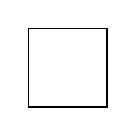
\begin{tikzpicture}[baseline=4mm]
\draw (0,0) -- (1,0) -- (1,1) -- (0,1) -- cycle; 
\end{tikzpicture}

\part[2] La figure qui correspond à la {\bf Sortie B} est la Figure 
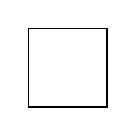
\begin{tikzpicture}[baseline=4mm]
\draw (0,0) -- (1,0) -- (1,1) -- (0,1) -- cycle; 
\end{tikzpicture}
\part[2] La figure qui correspond à la {\bf Sortie C} est la Figure 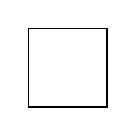
\begin{tikzpicture}[baseline=4mm]
\draw (0,0) -- (1,0) -- (1,1) -- (0,1) -- cycle; 
\end{tikzpicture}
\part[2] La figure qui correspond à la {\bf Sortie D} est la Figure 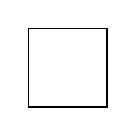
\begin{tikzpicture}[baseline=4mm]
\draw (0,0) -- (1,0) -- (1,1) -- (0,1) -- cycle; 
\end{tikzpicture}
\end{parts}
\begin{solution}
\begin{parts}
\part Figure 3
\part Figure 4
\part Figure 2
\part Figure 1
\end{parts}
\end{solution}

\newpage 

\question[9] Soit $X_1,\hdots, X_{36}$, des variables aléatoires indépendantes et identiquement distribuées selon une loi normale d'espérance~$\mu$ et de variance $\sigma^2=1296$.
On désire faire un \textbf{test unilatéral à droite} avec $H_0:\mu=10$ au seuil $\alpha = 0,025$.
On a les résultats suivants:
\begin{align*}
    \bar{x}= 11,34 &  & s^2=754.
\end{align*}
Si on sait qu'en réalité $\mu=\mu_1$ et que la puissance du test est $0,13567$, que vaut $\mu_1$? \textbf{\textit{Donnez les détails de votre démarche.}}

\begin{solution}
    La puissance est définie comme étant $1-\beta=P(Z_0>z_{\alpha}|\mu=\mu_1)$ qui est prob. de rejeter sachant que $H_0$ est fausse.

    \begin{align*}
        1-\beta &= P(Z_0>z_{\alpha}|\mu=\mu_1)\\
        0,13567&= P\left(\frac{\bar{X}-\mu_0}{\sigma/\sqrt{n}}>z_{\alpha}|\mu=\mu_1\right)\\
        0,13567&= P\left(\frac{\bar{X}-10}{36/6}>1,96|\mu=\mu_1\right)\\
        0,86433&= P\left(\frac{\bar{X}-10}{6}\leq1,96|\mu=\mu_1\right)\\
        0,86433&= P\left(\bar{X}\leq21,76|\mu=\mu_1\right)\\
        0,86433&=P\left(\frac{\bar{X}-\mu_1}{6}\leq\frac{21,76-\mu_1}{6}|\mu=\mu_1\right)\\
        0,86433&=P\left(Z\leq\frac{21,76-\mu_1}{6}|\mu=\mu_1\right)\\
    \end{align*}

Par la table de la loi normale centrée réduite, nous avons
\begin{align*}
    \frac{21,76-\mu_1}{6}=&1,1\\
    21,76-\mu_1=6,6\\
    \mu_1 =15,1
\end{align*}
\end{solution}
\newpage 

%%%%%%%%%%%%%%%% QUESTION %%%%%%%%%%%%%%%%
\question\label{test2variances}

On veut faire le test d'hypothèse suivant 
\begin{align*}
H_0 &:\sigma_1^2 = \sigma_2^2\\
H_1 &:\sigma_1^2 \neq \sigma_2^2,
\end{align*}

où la variable 1 suit une loi normale de moyenne $\mu_1$ et de variance $\sigma_1^2$ et la variable 2 suit une loi normale de moyenne $\mu_2$ et de variance $\sigma_2^2$. On sélectionne aléatoirement 30 observations de la variable 1 et 30 observations de la variable 2 de façon indépendante. On obtient la sortie \texttt{Rcmdr} suivante où certaines valeurs ont été remplacées par \texttt{AAAA} et \texttt{BBBB}:

\begin{verbatim}
> var.test(x ~ obs, alternative='two.sided', conf.level=.95, data=donnees)

	F test to compare two variances

data:  x by obs
F = 0.15,   num df = AAAA,   denom df = BBBB,   p-value = 0.00000204
alternative hypothesis: true ratio of variances is not equal to 1
95 percent   confidence interval:
0.07139472   0.3151494
sample estimates:
ratio of variances 
0.15
\end{verbatim}

\begin{parts}
\part[2] Donnez la valeur de \texttt{AAAA}, soit le nombre de degrés de liberté associés au numérateur de la statistique de test. 

\vspace{1.8cm}

\part[2] Donnez la valeur de \texttt{BBBB}, soit le nombre de degrés de liberté associés au dénominateur de la statistique de test.

\vspace{1.8cm}

\part[3] On vous indique que la variance échantillonnale de la variable 1, $s_1^2$, vaut 6,69. Quelle est la valeur de la variance échantillonnale de la variable 2, soit $s_2^2$? \textit{\textbf{Donnez les détails de votre démarche.}}

\vspace{3.2cm}

\part[2] En utilisant l'information disponible dans la sortie \texttt{Rcmdr}, choisissez l'énoncé qui est vrai. 
	\begin{checkboxes}
		\CorrectChoice La variance de la variable 1 est significativement différente de celle de la variable~2 au seuil 5\%.
		\choice La variance de la variable 1 n'est pas significativement différente de celle de la variable~2 au seuil 5\%.
		\choice Au seuil 5\%, on ne peut rien conclure  à partir de la sortie \texttt{Rcmdr}.
	\end{checkboxes}
	

%\part[3] Si on avait choisi un niveau de confiance à 90\%, l'intervalle de confiance aurait été
%	\begin{checkboxes}
%		\choice plus long.
%		\CorrectChoice plus court.
%		\choice de même longueur.
%		\choice plus long ou plus court, on manque d'information pour le déterminer. 
%	\end{checkboxes}


\end{parts}

	\begin{solution}
		ZONE 1:  $n_1-1=30-1=29$\\
		ZONE 2:  $n_2-1=30-1=29$\\
		ZONE 3: $\displaystyle f_0= \frac{s_1^2}{s_2^2}$ alors
		$ \displaystyle s_2^2 = \frac{s_1}{f_0}
		= \frac{6,69}{0,15}
		= 44,60	$ \\
		ZONE 4: A. différent car valeur-p inférieure à 5\%.\\
%		ZONE 5:	Plus court. 
	\end{solution}

\newpage 

%%%%%%%%%%%%%%%% QUESTION %%%%%%%%%%%%%%%%
\question\label{rls}

Afin d'estimer le volume de bois disponible dans la forêt entre Burtigny et Saint-Oyens, on aimerait modéliser le volume de bois d'un arbre à l'aide de sa circonférence puisqu'il est beaucoup plus facile de mesurer la circonférence d'un arbre que sa hauteur. On dispose du volume ($Y$) et de la circonférence ($X$) de 31 arbres. Afin d'étudier le modèle $Y_i = \beta_0 + \beta_1 X_i + E_i$, en supposant que les postulats de régression linéaire sont respectés, vous disposez des résultats suivants:

\begin{verbatim}
Residual standard error: 4.252 on 29 degrees of freedom
Multiple R-squared:  0.9353,	 Adjusted R-squared:  0.9331 
F-statistic: 419.4 on 1 and 29 DF,  p-value:  0.00014
\end{verbatim}
\begin{align*}
	\sum_{i=1}^{31} x_i &= 410,70;  \quad \sum_{i=1}^{31} x_i^2 = 5\; 736,55 ; \quad \sum_{i=1}^{31} x_iy_i =13\; 887,86;\quad
	\sum_{i=1}^{31} y_i &= 935,30; \quad \sum_{i=1}^{31} y_i^2 = 36\; 324,99.
\end{align*}

\begin{parts}
	\part[7] Donnez l'équation de la droite de régression permettant de prédire le volume de bois d'un arbre de circonférence précise. \textbf{\textit{Donnez les détails de votre démarche.}}
	
	
	
	\begin{solution} $$ \widehat{\beta}_1 
		= \frac{S_{XY}}{S_{XX}}
		= \frac{\sum x_iy_i - n\overline{x}\overline{y}}{\sum x_i^2 - n\overline{x}^2} 
		= \frac{\displaystyle 13\; 887.86 -  \frac{410.7 \times  935.3}{31}}{\displaystyle 5\; 736.55 - \frac{410.7^2 }{ 31} }
		= \frac{1496.644}{295.4374}
		= 5.065858 $$
	
	$$ \widehat{\beta}_0 =  \overline{y}-\widehat{\beta}_1 \overline{x} 
		= \frac{935.3}{31} -  5.065858 \frac{410.7}{31} 
		= -36.94348 $$ 
		
		$$ \widehat{Y}_i = -36.94348 + 5.065858  x_i$$
		\end{solution}
\vspace{13cm}
    \part[2] Donnez le pourcentage de la variabilité totale du volume qui est expliquée par la circonférence. 
	

	
	\begin{solution}
	Multiple R-squared:  0.9353
	
	93,53\%
	\end{solution}
		\vspace{2cm}
	\pagesuivante{\ref{rls}}

\newpage 

\suite{\ref{rls}}

	\part[3] Calculez la prévision ponctuelle du volume de bois d'un arbre ayant une circonférence de 11. \textbf{\textit{Donnez les détails de votre démarche.}}
	

	
	\begin{solution}$$ \widehat{y}_i = \widehat{\beta}_0 + \widehat{\beta}_1 x_i
		= -36.94348 + 5.065858  \times 11 = 18.78096$$
		\end{solution}
		\vspace{4cm}


	\part[2] Gérard aimerait estimer le volume de bois de l'arbre devant sa maison. Cet arbre a une circonférence de 14. La prévision ponctuelle du volume de bois de cet arbre est environ 33.98. Choisissez l'intervalle de valeurs ayant 95\% de chances de contenir le volume de bois de cet arbre de circonférence 14.
	
	\begin{checkboxes}
			\choice $ \displaystyle	33.98 \pm t_{0,05;29} \sqrt{MS_E \left[ \frac{1}{n} + \frac{(14-\overline{x})^2}{S_{XX}}\right]} $ 
   \choice $ \displaystyle	33.98 \pm t_{0,025;1} \sqrt{MS_E \left[ \frac{1}{n} + \frac{(14-\overline{x})^2}{S_{XX}}\right]} $ 
   			\choice $ \displaystyle	33.98 \pm t_{0,025;29} \sqrt{MS_E \left[ \frac{1}{n} + \frac{(14-\overline{x})^2}{S_{XX}}\right]} $ \vspace{0.2cm}
			\correctchoice $ \displaystyle		33.98 \pm t_{0,025;29} \sqrt{MS_E \left[ 1+ \frac{1}{n} + \frac{(14-\overline{x})^2}{S_{XX}}\right]} $
   \choice $ \displaystyle		33.98 \pm t_{0,025;1} \sqrt{MS_E \left[ 1+ \frac{1}{n} + \frac{(14-\overline{x})^2}{S_{XX}}\right]} $
	\end{checkboxes}
\vspace{0.5cm}
		\part[1] Si Gérard avait un arbre ayant une circonférence de 18, l'intervalle de valeurs calculé à la question précédente serait... 
	\begin{checkboxes}
			\choice plus court 
			\choice de même longueur  
			\correctchoice plus long   
		\choice on ne peut pas savoir la différence de longueur 
	\end{checkboxes}
\vspace{0.5cm}

\part[2] Quelle affirmation parmi les suivantes est vraie au seuil 1\%? 
	\begin{checkboxes}
			\choice La circonférence d'un arbre et le volume de celui-ci ne sont pas unis par une relation linéaire significative. 
			\choice On ne peut pas prédire la valeur du volume de bois d'un arbre à partir de sa circonférence.
			\choice La circonférence d'un arbre et le volume de celui-ci sont indépendants.  
		\correctchoice La relation linéaire entre le volume de bois d'un arbre et sa circonférence est significative. 
	\end{checkboxes}

\end{parts}

\newpage
\question Supposons que les variables aléatoires $X_1,...,X_{20}$ suivent une loi exponentielle décalée de paramètre $\theta \geq0 $, dont la \textbf{fonction de densité} est donnée par 

 \begin{equation*}
  f_X(x) = \begin{cases}
         e^{-(x-\theta)},\ \text{  si  } \theta \leq x , \\
        0, \text{ sinon.}
        \end{cases}
 \end{equation*}

Nous aimerions faire un test statistique pour savoir si $\theta=0$. Nous avons donc les hypothèses

\begin{table}[ht]
    \centering
    \begin{tabular}{cc}
         $H_0: \theta=0$ & $H_1: \theta > 0$.
    \end{tabular}
\end{table}
Pour ce test, nous utiliserons la statistique
\begin{align*}
    M=\min (X_1,...,X_{20}),
\end{align*}
qui correspond à la valeur minimale de notre échantillon (nous pouvons aussi écrire $M=X_{(1)}$, dans la notation introduite au cours).
Nous savons que sous $H_0$, $M$ suit une loi exponentielle de paramètre $n=20$. Sa \textbf{fonction de répartition} est donnée par 

 \begin{equation*}
  F_M(m) = \begin{cases}
         1-e^{-20m},\ \text{  si  } 0\leq m \\
        0, \text{ sinon.}
        \end{cases}
 \end{equation*}

La table suivante donne quelques valeurs de cette fonction de répartition.
\begin{table}[ht]
    \centering
\begin{tabular}{|cc|}
  \hline
 $m$ & $F_M(m)$ \\ 
  \hline
    0,0005 & 0,01 \\
    0,0025 & 0,05 \\
    0,0053 & 0,10 \\
    0,1151 & 0,90 \\
    0,1498 & 0,95 \\ 
    0,2303 & 0,99 \\ 
  \hline
\end{tabular}
\end{table}

Nous avons l'échantillon $x_1,\hdots,x_{20}$ suivant:

\begin{table}[ht]
\centering
\begin{tabular}{rrrrrrrrrr}
  \hline
0,1613 & 0,1933 & 0,2980 & 0,3331 & 0,3423 & 0,4392 & 0,4472 & 0,4580 & 0,5289 & 0,5530 \\ 
0.5570 & 0.7737 & 0.8574 & 0.9376 & 1.2509 & 1.4475 & 1.9064 & 2.6019 & 2.8685 & 2.9829 \\ 
   \hline
\end{tabular}
\end{table}
\begin{parts}
\part[3] Au seuil $\alpha=5\%$, quelle est la \textit{\textbf{décision}} du test. \textbf{\textit{Une décision sans justification n'obtiendra aucun point, même si la décision est bonne.}}
\vspace{3cm}
\part[3] \textbf{Calculez} la valeur-p du test en ne gardant que 4 chiffres après la virgule. \textit{\textbf{Expliquez votre réponse!}}
\end{parts}

\begin{align*}
    b_1\pm& t_{\alpha/2;n-2}\sqrt{\frac{\sum(y_i-\hat{y_i})^2}{(n-2)\sum(x_i-\Bar{x})^2}}\\
    31,65 \pm& 2,160 \sqrt{\frac{3,91}{133668,3}}

\end{align*}
\end{questions}

\end{document} 

\newpage
%%%%%%%%%%%%%%%% TABLES DE LOIS %%%%%%%%%%%%%%%%

\begin{center}

\includegraphics[page=1,scale=0.8]{Tables_lois.pdf}
\end{center}

\begin{center}

\includegraphics[page=2,scale=0.8]{Tables_lois.pdf}
\end{center}

\begin{center}

\includegraphics[page=3,scale=0.8]{Tables_lois.pdf}
\end{center}
\begin{center}


\includegraphics[page=4,scale=0.8]{Tables_lois.pdf}
\end{center}
\begin{center}


\includegraphics[page=5,scale=0.8]{Tables_lois.pdf}
\end{center}
\begin{center}


\includegraphics[page=6,scale=0.8]{Tables_lois.pdf}
\end{center}
\begin{center}


\includegraphics[page=7,scale=0.8]{Tables_lois.pdf}
\end{center}
\begin{center}


\includegraphics[page=8,scale=0.8]{Tables_lois.pdf}
\end{center}







%\newpage
%\mbox{}
%\newpage


%%%%%%%%%%%%%%%% QUESTION SPPLÉMENTAIRE %%%%%%%%%%%%%%%%
%\question\label{cable} 


%La société ROULEMENTABILLE fabrique des roulements à billes. Les tolérances exigées pour un client, la DUPONT S.A., sont particulièrement draconiennes. Pour cette raison, un contrôle de qualité est effectué sur chaque bille avant livraison. La proportion de pièces ne satisfaisant pas aux spécifications de diamètre est de 10\% et la proportion de pièces présentant un défaut de forme est de 20\%.\\

%\begin{parts}
%\part[] Question a.

    %\bigskip

    %Le chef d'atelier estime que ces deux types de défaut sont indépendants. Si l'on suppose qu'il a raison, quelle est la proportion de pièces présentant au moins un défaut?

%\begin{solution}
%\begin{itemize}\itemsep10pt
       % \item[$\bullet$] Soient les événements $A$ = "défaut de diamètre" et $B$ = "défaut de forme".
      %  \item[$\bullet$] On sait que: $P(A) = 0.1,\; P(B) = 0.2$,\\ \ \\
      %   alors $P(A \cap B) = P(A) \times P(B)$ (car $A$ et $B$ sont supposés indépendants).
     %    Donc, \begin{eqnarray*}
      %            P(A \cup B)  &=& P(A) + P(B) - P(A \cap B) \\
     %             &=& P(A) + P(B) – P(A) \times P(B) \\
      %            &=& 0.1 + 0.2 – (0.1 \times 0.2) \\
      %            &=&  0.28.
     %          \end{eqnarray*}
  %  \end{itemize}
 %   La proportion de pièces présentant au moins un défaut est de \textbf{28\%}.
%\end{solution}


%\vspace{1cm}
%\part[] Question b.

\bigskip
%Le directeur de la fabrication n'est pas d'accord. Lorsque les pièces présentent un défaut de forme, alors dans 30\% des cas les pièces présentent un diamètre non conforme aux spécifications. Si l'on suppose que le directeur a raison, quelle est la nouvelle proportion de pièces présentant au moins un défaut?    

%\begin{solution}
%\begin{itemize}\itemsep10pt
 %           \item[$\bullet$] On nous indique que $P(A | B) = 0.3$. Alors,
 %                           \begin{eqnarray*}
  %                            P(A \cap B)  &=& P(A | B) \times P(B) \\
   %                                     &=& 0.3 \times 0.2 \\
    %                                    &=& 0.06
     %                       \end{eqnarray*}
      %       À la lumière de cette nouvelle information, On recalcule $P(A \cup B)$:
       %                     \begin{eqnarray*}
        %                      P(A \cup B)  &=& P(A) + P(B) - P(A \cap B) \\
         %                               &=& 0.1 + 0.2 – 0.06 \\
          %                              &=& 0.24
           %                 \end{eqnarray*}
        %\end{itemize}
       % La proportion de pièces présentant au moins un défaut est de \textbf{24\%}.
%\end{solution}


%\end{parts}


%\newpage
%\mbox{}
%\newpage

%\end{questions}



%%%%%%%%%%%%%%%% QUESTION %%%%%%%%%%%%%%%%
\question[3]\label{probabilite} 

On considère une expérience aléatoire dont deux événements  $A$ et $B$ sont tels que:\\ $P(A) = 0.3 \text{ et } P(A \cup B) = 0.7$.\\ 

Calculer $P(\overline{B}|\overline{A})$. Justifiez votre réponse.\\

\emptybox{15cm}

\begin{solution}
\begin{eqnarray*}
   P(\overline{B}|\overline{A})      &=&  \dfrac{P(\overline{B}\cap \overline{A})}{P(\overline{A})}\\
                                    &=&  \dfrac{P(\overline{B\cup A})}{1-P(A)}\\
                                    &=&  \dfrac{1-P(B\cup A)}{1-P(A)}\\
                                    &=&  \dfrac{1-0.7}{1-0.3}\\
                                    &=&  \dfrac{3}{7} .
\end{eqnarray*}
\end{solution}




\newpage